%%%%%%%%%%%%%%%%%%%%%%%%%%%%%%%%%%%%%%%%%
% Beamer Presentation
% LaTeX Template
% Version 1.0 (10/11/12)
%
% This template has been downloaded from:
% http://www.LaTeXTemplates.com
%
% License:
% CC BY-NC-SA 3.0 (http://creativecommons.org/licenses/by-nc-sa/3.0/)
%
%%%%%%%%%%%%%%%%%%%%%%%%%%%%%%%%%%%%%%%%%

%----------------------------------------------------------------------------------------
%	PACKAGES AND THEMES
%----------------------------------------------------------------------------------------

\documentclass[aspectratio=169]{beamer}
\usetheme[progressbar=frametitle]{metropolis}
\usepackage{appendixnumberbeamer}


\mode<presentation> {

% The Beamer class comes with a number of default slide themes
% which change the colors and layouts of slides. Below this is a list
% of all the themes, uncomment each in turn to see what they look like.

%\usetheme{default}
%\usetheme{AnnArbor}
%\usetheme{Antibes} 
%\usetheme{Bergen}
%\usetheme{Berkeley}
%\usetheme{Berlin}
% \usetheme{Boadilla} %
%\usetheme{CambridgeUS} %
%\usetheme{Copenhagen}
%\usetheme{Darmstadt}
%\usetheme{Dresden}
%\usetheme{Frankfurt}
%\usetheme{Goettingen}
%\usetheme{Hannover}
%\usetheme{Ilmenau}
%\usetheme{JuanLesPins}
%\usetheme{Luebeck}
%\usetheme{Madrid} %
%\usetheme{Malmoe}
%\usetheme{Marburg}
%\usetheme{Montpellier}
%\usetheme{PaloAlto}
%\usetheme{Pittsburgh}
%\usetheme{Rochester}
%\usetheme{Singapore} %
%\usetheme{Szeged}
%\usetheme{Warsaw}

% As well as themes, the Beamer class has a number of color themes
% for any slide theme. Uncomment each of these in turn to see how it
% changes the colors of your current slide theme.

%\usecolortheme{albatross}
%\usecolortheme{beaver} %
%\usecolortheme{beetle}
%\usecolortheme{crane}
%\usecolortheme{dolphin}
%\usecolortheme{dove}
%\usecolortheme{fly}
%\usecolortheme{lily}
%\usecolortheme{orchid}
%\usecolortheme{rose}
%\usecolortheme{seagull}
%\usecolortheme{seahorse}
%\usecolortheme{whale}
%\usecolortheme{wolverine}

%\setbeamertemplate{footline} % To remove the footer line in all slides uncomment this line
%\setbeamertemplate{footline}[page number] % To replace the footer line in all slides with a simple slide count uncomment this line

\setbeamertemplate{navigation symbols}{} % To remove the navigation symbols from the bottom of all slides uncomment this line
}

\usepackage{graphicx} % Allows including images
\usepackage{booktabs} % Allows the use of \toprule, \midrule and \bottomrule in tables

\usepackage{accents}
\newcommand{\ubar}[1]{\underaccent{\bar}{#1}}
\usepackage{stmaryrd}


\usepackage{pgfplots}
\pgfplotsset{width=7cm,compat=1.9}

\usepackage{tabularx}
\newcolumntype{Y}{>{\centering\arraybackslash}X}\newcolumntype{Y}{>{\centering\arraybackslash}X}
	\newcommand\fnote[1]{\captionsetup{font=footnotesize}\caption*{#1}}
	\newcolumntype{K}[1]{>{\centering\arraybackslash}p{#1}}
\newcolumntype{P}[1]{>{\centering\arraybackslash}p{#1}}

\usepackage{amssymb}
\usepackage{amsmath}

% Add significance note with \starnote
\newcommand{\starnote}{\figtext{* p $<$ 0.1, ** p $<$ 0.05, *** p $<$ 0.01. Standard errors in parentheses.}}

\usepackage{siunitx} % centering in tables
\sisetup{
detect-mode,
tight-spacing		= true,
group-digits		= false ,
input-signs		= ,
input-symbols		= ( ) [ ] - + *,
input-open-uncertainty	= ,
input-close-uncertainty	= ,
table-align-text-post	= false
        }
\makeatother

%----------------------------------------------------------------------------------------
%	TITLE PAGE
%----------------------------------------------------------------------------------------

\title[Continuous Survey Sample Optimization]{Continuous Survey Sample Optimization \\ Using Ad Platform APIs} % The short title appears at the bottom of every slide, the full title is only on the title page

% Authors
\author[Nandan Rao]{Nandan Rao \inst{1} \and Dante Donati \inst{2}}
% Affiliations
\institute[Virtual Lab]{\inst{1} Virtual Lab and UAB \and \inst{2} Columbia University}


\date[\today] {\today} % Date, can be changed to a custom date

\begin{document}

\begin{frame}
\titlepage % Print the title page as the first slide
\end{frame}


%----------------------------------------------------------------------------------------
%	PRESENTATION SLIDES
%----------------------------------------------------------------------------------------

%------------------------------------------------
\section{Introduction}
\begin{frame}
\frametitle{Motivation}
\begin{itemize}
\item<1-> Online marketplaces such as eBay, Amazon, Airbnb, Uber and Etsy are booming
%are one of the greatest success stories of the internet over the past two decades
	\begin{itemize}
		\vspace{.5mm}
	\item Create new markets and business opportunities
		%\vspace{.5mm}
	%\item Save sellers from extra costs to market their products
		\vspace{.5mm}
	\item Help \textbf{match demand with supply} efficiently
	\end{itemize}
	
	\vspace{4mm}
\item<2->  \textbf{Reputation systems} play a \textbf{central role} (Tadelis 2016)
	\begin{itemize}
		\vspace{.5mm}
	\item Reviews from users alleviate asymmetric information and allow markets to exist
	\end{itemize}
	
	\vspace{4mm}
	
\item<3-> Review platforms such as \textbf{Tripadvisor} and Yelp enter existing markets with serious \textbf{information problems} (e.g., experience goods)
\begin{itemize}
		\vspace{.5mm}
	\item Unobserved quality $\Rightarrow$ welfare losses for consumers/producers (Akerlof 1970; Leland 1979)	
		\vspace{.5mm}
	\item Repeat purchases, chain affiliation (brand) and regulation offer only a partial solution
	\end{itemize}
\end{itemize}
\end{frame}

%------------------------------------------------

\begin{frame}
\frametitle{This paper}
\begin{itemize}

\item<1-> Derives hypotheses from model: \textbf{$\downarrow$ consumer search costs $\Rightarrow$}

\begin{itemize}
\item[\textbf{1.}]Firms with \textit{ex-ante} higher-qualities $\uparrow$ output
\vspace{1mm}
\item[\textbf{2.}]Lowest-quality firms exit the market
\vspace{1mm}
\item[\textbf{3.}] Operating firms $\uparrow$ qualities,  especially those selling \textit{ex-ante} lower-quality products
\end{itemize}


\vspace{3mm}

\item<2-> Empirically tests these predictions

\begin{itemize}
\item 5,500 restaurants in Rome %($\sim$ 5\% of the total labor force)
\vspace{1mm}
\item \textbf{Natural experiment} (roaming charges in the EU) $\downarrow$ costs to access online info for tourists
\vspace{1mm}
\item \textbf{Novel dataset} linking Tripadvisor data with restricted-use employer-employee records
\vspace{1mm}
\item Diff-in-Diff strategy: pre/post policy $\times$ more/less tourist exposure
	\end{itemize}
	
\vspace{3mm}

\item<3> Estimates the impact of \textbf{access to online reviews} on 
\begin{itemize}
	\item Revenues and total employment (output)
	\vspace{1mm}
	\item Production costs, hiring decisions and online ratings (quality upgrading)
	\end{itemize}

\end{itemize}
\end{frame}
%------------------------------------------------
\section{Literature}

\begin{frame}
\frametitle{Related literature and contribution}

\begin{itemize}

\item<1-> Review platforms and economic outcomes
\begin{itemize}
\item Online reputation is a significant driver of sales \textcolor{gray}{\scriptsize (Chevalier and Mayzlin 2006; Cabral and Hortacsu 2010; Anderson and Magruder 2012, Luca 2016)}
\item  Online reputation and firms' strategic use of management responses and advertising spending \textcolor{gray}{\scriptsize (Hollenbeck et al. 2019; Chevalier et al.  2018; Proserpio and Zervas 2017)}
\item Disclosure and quality choices \textcolor{gray}{\scriptsize (Ananthakrishnan et al. 2019; Farronato and Zervas 2019)}
\vspace*{-1ex}
\begin{block}{\vspace{-3ex}}
\textbf{Novel data on firm-specific production/employment choices to proxy for quality upgrading}
\end{block}

\end{itemize}

\vspace{3mm}

\item<2> Information and product quality
\begin{itemize}

\item Theoretically,  information to consumers $\rightarrow$ firms choices on entry, pricing, quality and product design \textcolor{gray}{\scriptsize (Goldmanis et al. 2010; Bar-Isaac et al. 2012; Fishman et al. 2015)}

%(hygiene grade cards)
\item Quality disclosure programs and increased transparency in online markets $\rightarrow$ consumers and producers' behavior \textcolor{gray}{\scriptsize (Jin and Leslie 2003, Dranove and Jin 2010, Klein et al. 2016, Hui et al. 2018, 2020)}
\vspace*{-1ex}
\begin{block}{\vspace{-3ex}}
\textbf{Broader policy to study the general equilibrium effects of information from online reviews}
\end{block}
\end{itemize}

\end{itemize}
\end{frame}




%------------------------------------------------
\section{Empirics}

\begin{frame}[noframenumbering]
\Huge{\centerline{Empirical Framework}}

\vspace{5mm}

\begin{figure}[H]
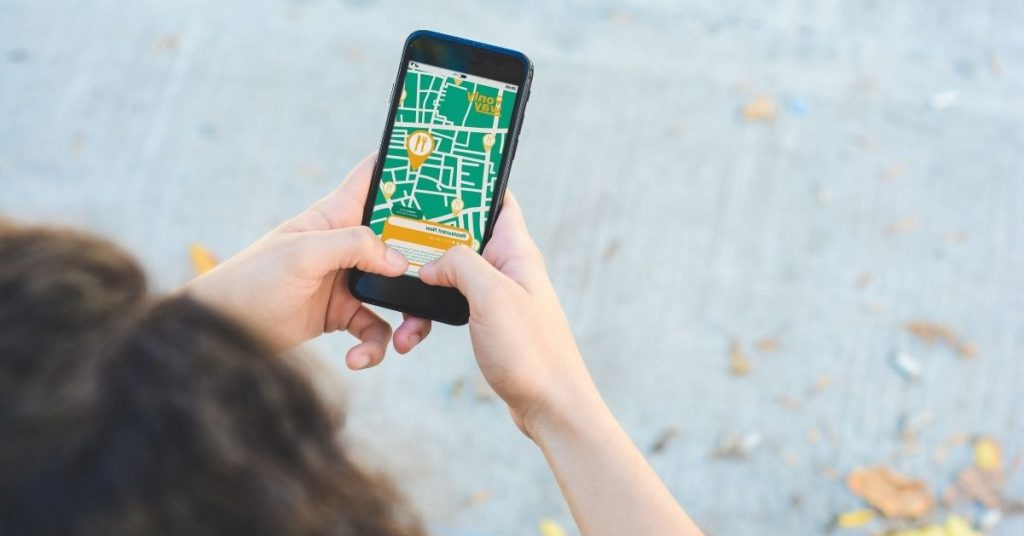
\includegraphics[scale=0.35]{Figures/TripAdvisor-1024x536.jpeg} 
\end{figure}
\end{frame}





%------------------------------------------------
\begin{frame}
\frametitle{Identification strategy}
\begin{itemize}
\item<1-> \textbf{Difference-in-Differences:} I compare changes (before/after policy) in the outcomes of interest across restaurants that are differentially exposed to tourist clientele:

\[y_{i,t}=\beta Tourist_{i}\times Post_{t}+\alpha_{i}+\gamma_{t}+\phi \mathbf{x}_{i}\times Post_{t}+\varepsilon_{i,t}\]

\begin{itemize}

\item $Tourist$ is a binary variable = 1 if restaurant $i$ has a probability of being exposed to tourists $\geq$ median (I also use deciles/quintiles of probability)

\item $Post$ = 1 for time $t$ after May 2017 


%\item Controls: neighborhood time trends,  distance to the attraction,  price category, among others 

\item Estimation via OLS, standard errors clustered at the municipality level (86 clusters)


\end{itemize}

\vspace{2.5mm}
\item<2> \textbf{Identifying assumption:} changes in the outcomes across restaurants more and less exposed to tourists would have been the same in the absence of the policy

\begin{itemize}
%\item Plot averages and event-study estimates for pre-trends
\item Placebo exercises
\end{itemize}

\end{itemize}

\end{frame}

%------------------------------------------------
\section{Results}

\begin{frame}[noframenumbering]
\Huge{\centerline{Results}}
\end{frame}

%------------------------------------------------
\begin{frame}[label=employees_fig]
\frametitle{Restaurants' employment}

\begin{itemize}
\item<1-> Consumers reallocate their demand towards higher-quality producers, which  expand their revenues and total employment \hyperlink{employees_eq}{\beamerskipbutton{Estimates}}
\end{itemize}

\begin{figure}[H]\centering
\label{fig:f3}
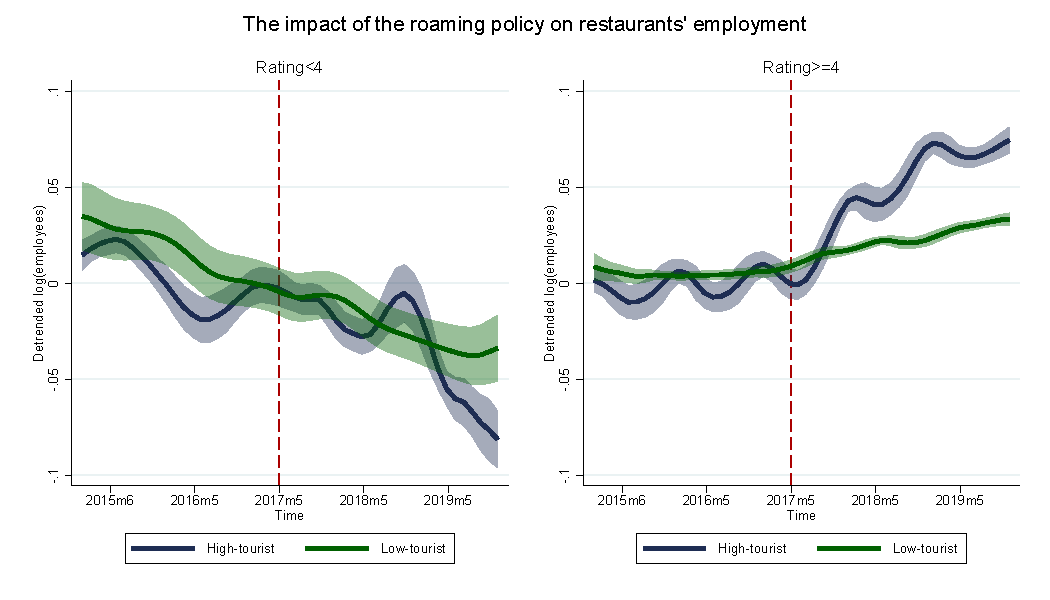
\includegraphics[scale=0.62]{Figures/new_g4.pdf} 
\begin{minipage}{0.8\textwidth} % choose width suitably
{\tiny Data on $\sim$5,000 matched restaurants.  Lines represent local polynomial fits of monthly averages with 95\% confidence intervals.\par}
\end{minipage}
\end{figure} 

\end{frame}

%------------------------------------------------

\section{Conclusions}

\begin{frame}[label=conclusions]
\frametitle{Conclusions}
\begin{itemize}

\item<1-> Review platforms can complement conventional programs (e.g., hygiene inspections) aimed at informing consumers and improving product quality  
%and advertising)  and strategies 
%Crowd-sourced information from review platforms matters!
\vspace{3.5mm}

\item<2->[\textbf{1.}] \textbf{Consumers learn}
 \begin{itemize}
\item Better-rated restaurants $\uparrow$ revenues and total employment
\end{itemize}


\vspace{3mm}

 \item<2->[\textbf{2.}]   \textbf{Industry composition changes}
 \begin{itemize}
\item Share of lowest-rated restaurants in the most tourist areas $\downarrow$ by $\sim$2.5 pp
\end{itemize}


\vspace{3mm}

\item<2->[\textbf{3.}]  \textbf{Average service quality $\uparrow$}

\begin{itemize}
\item Lower-rated restaurants hire more experienced workers with higher wages
\vspace{0.5mm}
\item Their Tripadvisor ratings improve over time
\end{itemize}

\end{itemize}

\end{frame}

%------------------------------------------------

{
\usebackgroundtemplate{%
\tikz[overlay,remember picture] \node[opacity=0.80, at=(current page.north)] [yshift = -4.3cm] {
   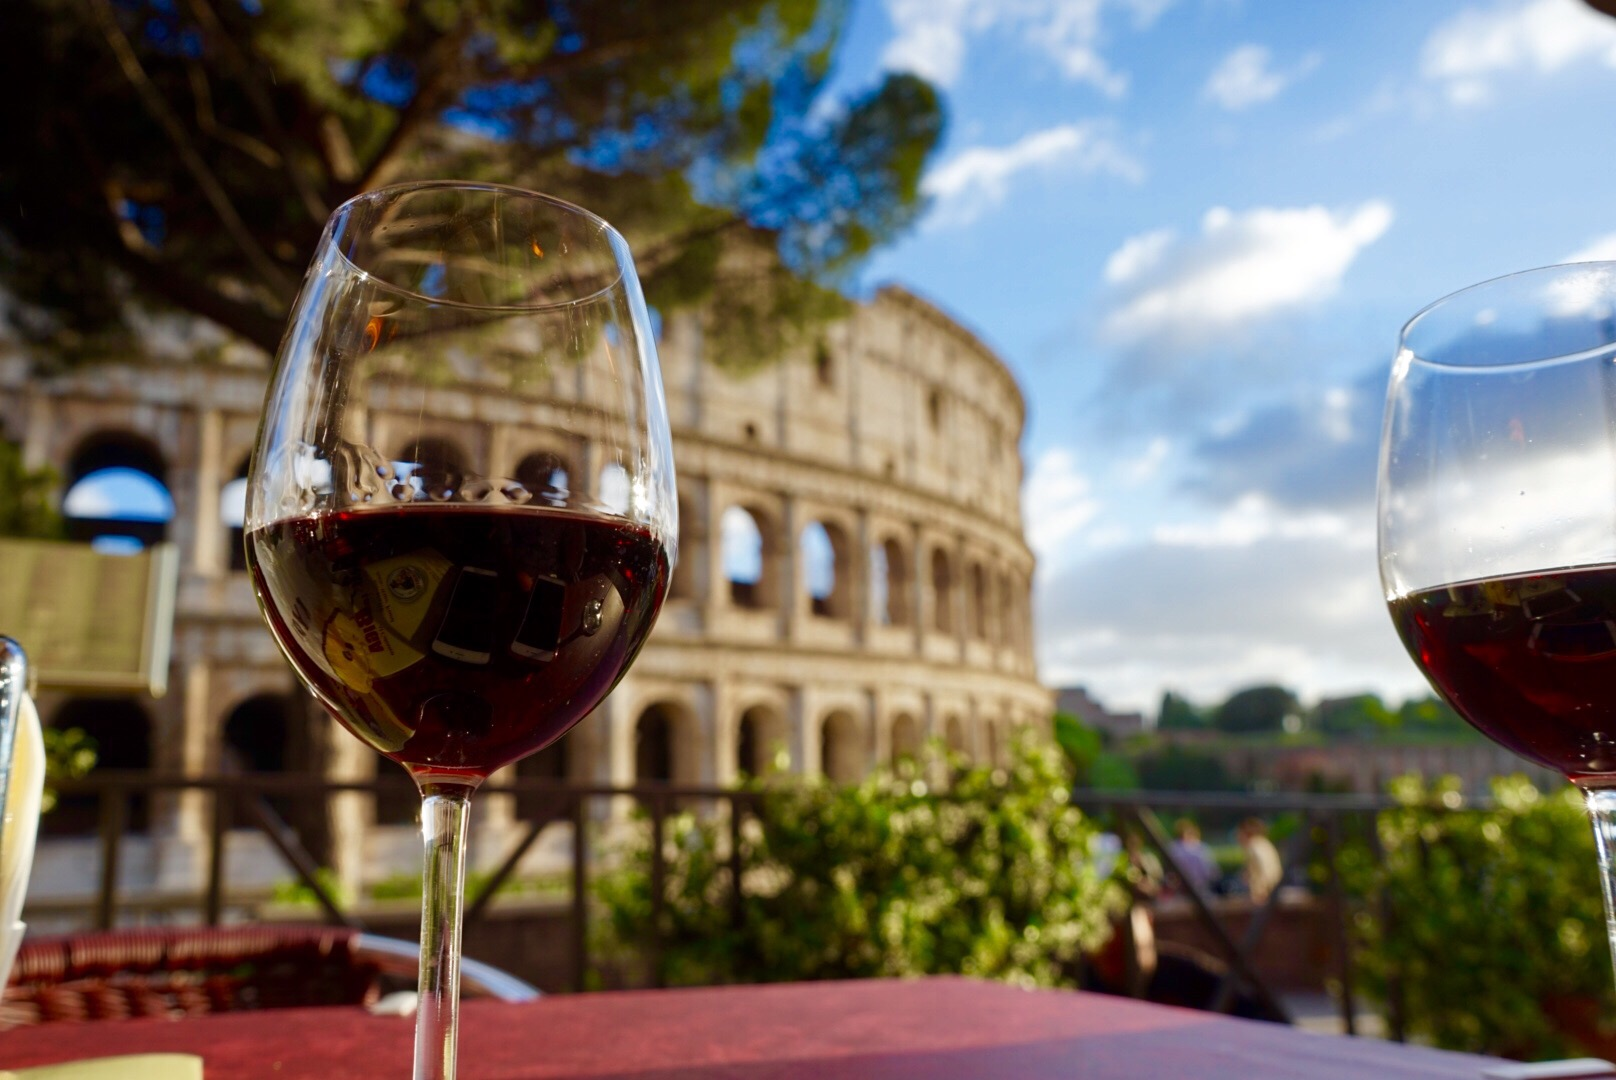
\includegraphics[width=\paperwidth  ]{Figures/last2.jpeg}};
}
\begin{frame}

\Huge{\centerline{Thank you!}}
\vspace{15mm}
\end{frame}
}

%------------------------------------------------
\appendix
\section{Appendix}
\begin{frame}[noframenumbering]
\Huge{\centerline{Appendix}}
\end{frame}
%------------------------------------------------

\begin{frame}[label=employees_eq,  noframenumbering]
\frametitle{Restaurant output: total employment}

\begin{table}[H]\centering
\def\sym#1{\ifmmode^{#1}\else\(^{#1}\)\fi}
\scriptsize
\begin{tabularx}{0.9\linewidth}{p{3.7cm} Y Y Y Y}
\hline\hline
                    &\multicolumn{4}{c}{Dependent variable: log(employees)}                                                       \\\cmidrule(lr){2-5}
                    &\multicolumn{1}{c}{(1)}         &\multicolumn{1}{c}{(2)}        &\multicolumn{1}{c}{(3)}         &\multicolumn{1}{c}{(4)}         \\
                    & Full sample         & Full sample             &   Rating$\geq$4         &    Rating$<$4         \\
\hline
Tourist*Post        &       0.043\sym{***}&       0.037\sym{**} &            0.063\sym{***}&      -0.042\sym{*}  \\
                    &     (0.011)         &     (0.015)              &     (0.023)         &     (0.024)         \\
Restaurant FE       &$\checkmark$         &$\checkmark$               &$\checkmark$         &$\checkmark$         \\
Month+Year FE       &$\checkmark$         &$\checkmark$             &$\checkmark$         &$\checkmark$         \\
Neighborhood*Time&$\checkmark$         &$\checkmark$               &$\checkmark$         &$\checkmark$         \\
Controls            &$\checkmark$         &$\checkmark$               &$\checkmark$         &$\checkmark$         \\
Extra controls      &                     &$\checkmark$                &$\checkmark$         &$\checkmark$         \\
\hline
Observations        &\num{223448}         &\num{210774}             &\num{153479}         & \num{57295}         \\
Restaurants         &        4632         &        4333                &        3186         &        1147         \\
Clusters            &          86         &          86              &          85         &          53         \\
Adj. R-squared      &       0.821         &       0.823               &       0.818         &       0.824         \\
Mean Y before policy&         6.8         &         7.0              &         5.8         &        10.1         \\
\hline\hline
\multicolumn{5}{p{0.88\linewidth}}{\tiny Post=1 if date is after May 2017. Tourist restaurants are those with probability$\geq$1\%. Heteroskedasticity-robust standard errors clustered at municipality level. Each observation is a restaurant-month-year. Controls include (log) distance to closest attraction and (log) n. of attractions in 600m radius interacted with Post. Extra controls include: restaurant price category, indicator for Italian cuisine, indicator for TA profile managed by restaurant, n. of reviews to closest attraction, n. of restaurants in 400m radius, indicators for type of matching, main economic activity and legal status of the company. \sym{*} \(p<0.1\), \sym{**} \(p<0.05\), \sym{***} \(p<0.01\)}\\
\end{tabularx}
\end{table}

\hyperlink{employees_fig}{\beamerskipbutton{Back}}
\end{frame}

\end{document} 

%------------------------------------------------
